\documentclass[12pt,a4paper,oneside]{report}

% ---------------------------------------------------------
% Packages & Configuration
% ---------------------------------------------------------
\usepackage[utf8]{inputenc}
\usepackage[margin=1in, top=1in, bottom=1in, left=1.25in, right=1in]{geometry}
\usepackage{graphicx}
\graphicspath{{./}{report/}}
\usepackage{amsmath,amssymb}
\usepackage{booktabs}
\usepackage{tabularx}
\usepackage{enumitem}
\usepackage{caption}
\usepackage{subcaption}
\usepackage{titlesec}
\usepackage{fancyhdr}
\usepackage{listings}
\usepackage{xcolor}
\usepackage{tikz}
\usetikzlibrary{shapes.geometric, arrows, arrows.meta, positioning, fit, backgrounds, calc}
\usepackage{pgfgantt}
\usepackage{float}
\usepackage{cite}
\usepackage{url}
\usepackage[hidelinks, pdftex, pdfauthor={Student Name}, pdftitle={Orient Computer E-commerce Website Report}]{hyperref}

% ---------------------------------------------------------
% Code Listing Styling
% ---------------------------------------------------------
\definecolor{codegreen}{rgb}{0,0.6,0}
\definecolor{codegray}{rgb}{0.5,0.5,0.5}
\definecolor{codepurple}{rgb}{0.58,0,0.82}
\definecolor{backcolour}{rgb}{0.96,0.96,0.96}
\definecolor{orientblue}{RGB}{30,80,160}
\definecolor{orientred}{RGB}{200,40,40}
\definecolor{successgreen}{RGB}{39,174,96}

\lstdefinestyle{mystyle}{
    backgroundcolor=\color{backcolour},
    commentstyle=\color{codegreen},
    keywordstyle=\color{magenta},
    numberstyle=\tiny\color{codegray},
    stringstyle=\color{codepurple},
    basicstyle=\ttfamily\footnotesize,
    breakatwhitespace=false,
    breaklines=true,
    captionpos=b,
    keepspaces=true,
    numbers=left,
    numbersep=5pt,
    showspaces=false,
    showstringspaces=false,
    showtabs=false,
    tabsize=2
}
\lstset{style=mystyle}

% JavaScript language definition
\lstdefinelanguage{JavaScript}{
  keywords={typeof,new,true,false,catch,function,return,null,switch,var,if,in,while,do,else,case,break,const,let,async,await,export,import,from,of,class,extends,this,try,throw},
  keywordstyle=\color{orientblue}\bfseries,
  identifierstyle=\color{black},
  sensitive=false,
  comment=[l]{//},
  morecomment=[s]{/*}{*/},
  commentstyle=\color{codegreen}\ttfamily,
  stringstyle=\color{codepurple}\ttfamily,
  morestring=[b]',
  morestring=[b]",
  morestring=[b]`
}

% ---------------------------------------------------------
% Header & Footer Formatting
% ---------------------------------------------------------
\pagestyle{fancy}
\fancyhf{}
\fancyhead[L]{\small\nouppercase{\leftmark}}
\fancyhead[R]{\small Orient Computer E-commerce Website}
\fancyfoot[C]{\thepage}
\renewcommand{\headrulewidth}{0.4pt}
\renewcommand{\footrulewidth}{0pt}

\titleformat{\chapter}[display]
  {\normalfont\huge\bfseries}{\chaptertitlename\ \thechapter}{18pt}{\Huge}
\titlespacing*{\chapter}{0pt}{10pt}{20pt}

% ---------------------------------------------------------
% Variables
% ---------------------------------------------------------
\newcommand{\projectTitle}{Orient Computer E-commerce Website}
\newcommand{\studentName}{Sultana Tasnim Riza}
\newcommand{\studentId}{2111329}
\newcommand{\academicSupervisor}{Bijoy Rahman Arif}
\newcommand{\academicSupervisorTitle}{Senior Lecturer}
\newcommand{\industrySupervisor}{Md Sabbir Hasan Khan}
\newcommand{\industryCompany}{Orient Computers}
\newcommand{\submissionSemester}{Summer 2026}
\newcommand{\submissionDate}{12 September, 2026}
\newcommand{\departmentName}{Department of Computer Science \& Engineering}
\newcommand{\schoolName}{School of Engineering and Computer Science}
\newcommand{\universityName}{Independent University, Bangladesh}

\begin{document}

% =========================================================
% FRONT MATTER
% =========================================================
\pagenumbering{roman}

% ---------------------------------------------------------
% 1. Title Page
% ---------------------------------------------------------
\begin{titlepage}
    \centering
    \vspace*{0.5cm}

    
\begin{tikzpicture}[scale=0.8]
        \draw[thick, fill=blue!10] (0,0) circle (1.4cm);
        \draw[thick, fill=red!20] (0,0.2) -- (-0.6,-0.6) -- (0.6,-0.6) -- cycle;
        \node at (0, -0.2) {\textbf{\large IUB}};
        \node at (0, -1.8) {\small \textbf{INDEPENDENT UNIVERSITY}};
    \end{tikzpicture}

    \vspace{1.2cm}
    {\Large \textbf{An Undergraduate Internship Project on}}\\[0.4cm]
    {\LARGE \textbf{\projectTitle}}\\[1.2cm]

    {\large By}\\[0.4cm]
    {\Large \textbf{\studentName}}\\[0.2cm]
    {\large Student ID: \studentId}\\[1.0cm]

    {\large \textbf{\submissionSemester}}\\[1.2cm]

    {\large Supervisor:}\\[0.2cm]
    {\large \textbf{\academicSupervisor}}\\[0.15cm]
    {\small \academicSupervisorTitle}\\[0.15cm]
    {\small \departmentName}\\[0.15cm]
    {\small \universityName}\\[1.2cm]

    {\large \textbf{\submissionDate}}\\[1.2cm]

    {\small \textit{Dissertation submitted in partial fulfillment for the degree of Bachelor of Science in Computer Science}}\\[0.4cm]
    {\small \departmentName}\\[0.15cm]
    {\small \universityName}

    \vfill
\end{titlepage}

% ---------------------------------------------------------
% 2. Attestation
% ---------------------------------------------------------
\newpage
\chapter*{Attestation}
\addcontentsline{toc}{chapter}{Attestation}

I, \textbf{\studentName}, ID: \textbf{\studentId}, hereby declare that the report titled \textbf{``\projectTitle''} submitted in partial fulfillment of the requirement for the Degree of Bachelor of Science in Computer Science is the result of my own work. I also confirm that the work was carried out as a student of \universityName.

\vspace{0.4cm}
I would like to acknowledge the guidance of my supervisor, \academicSupervisor, who supported me throughout this project. I also declare that this work represents my personal understanding and the outcomes I achieved during my internship period.

\vspace{0.4cm}
The report also properly cites and credits all sources used for further inquiry about this report, contacting my supervisor in the internship setting, \industrySupervisor\ at \industryCompany\ through official communication channels.

\vspace{4.0cm}
\noindent
\begin{tabular}{ll}
\makebox[2.8in]{\hrulefill} & \makebox[2.8in]{\hrulefill} \\
Signature & Date \\[1.5cm]
\makebox[2.8in]{\textbf{\studentName}} & \\
Name &
\end{tabular}

\vfill
\begin{center}\small i\end{center}

% ---------------------------------------------------------
% 3. Acknowledgement
% ---------------------------------------------------------
\newpage
\chapter*{Acknowledgement}
\addcontentsline{toc}{chapter}{Acknowledgement}

I am grateful for the opportunity to complete this internship and produce the project described in this report. My thanks go first to the Almighty and to my family, who were patient and encouraging throughout the long hours of software development, debugging, and report writing.

\vspace{0.4cm}
My academic supervisor, \textbf{\academicSupervisor}, provided clear direction and asked the right questions at each review milestone. Without those check-ins the project would have drifted in several unhelpful directions.

\vspace{0.4cm}
I also thank the team at \textbf{\industryCompany}, particularly \textbf{\industrySupervisor}, for explaining the business requirements honestly. He helped me understand how orders are fulfilled, how district-wise delivery charges work in Bangladesh, and how manual bKash and Nagad payment verification is handled. His guidance encouraged me to work more carefully and confidently.

\vspace{0.4cm}
I express my sincere gratitude to the faculty members of the \departmentName\ at \universityName\ for establishing strong foundational concepts in web application design, data structures, and database management systems.

\vfill
\begin{center}\small ii\end{center}

% ---------------------------------------------------------
% 4. Letter of Transmittal
% ---------------------------------------------------------
\newpage
\chapter*{Letter of Transmittal}
\addcontentsline{toc}{chapter}{Letter of Transmittal}

\noindent
\submissionDate \\[0.3cm]
\textbf{\academicSupervisor} \\
\academicSupervisorTitle \\
\departmentName, \schoolName \\
\universityName \\[0.4cm]
\textbf{Subject: Submission of an internship report for graduation completion} \\[0.4cm]
Dear Sir,

\vspace{0.3cm}
I am submitting my Internship Report as part of the Bachelor Program in Computer Science. I am grateful for your supervision during my internship at \industryCompany, where I worked for three months under the guidance of \industrySupervisor.

\vspace{0.3cm}
The project involved designing and building a full-stack e-commerce web application for Orient Computer, a computer hardware and electronics retailer based in Dhaka, Bangladesh. The application lets customers browse products, place orders, and pay using Cash on Delivery, bKash, or Nagad. An administrative dashboard allows staff to manage the full order lifecycle including payment verification, product cataloging, stock control, and localized shipping fees.

\vspace{0.3cm}
I have tried to document the work clearly, including the decisions I made, the problems I faced, and how I solved them. If any section needs clarification, I would be happy to discuss it.

\vspace{0.3cm}
Thank you for your valuable guidance and consideration.

\vspace{1.5cm}
\noindent
Yours sincerely,\\[0.8cm]
\textbf{\studentName} \\
ID: \studentId \\
\departmentName, \\
\universityName

\vfill
\begin{center}\small iii\end{center}

% ---------------------------------------------------------
% 5. Evaluation Committee
% ---------------------------------------------------------
\newpage
\chapter*{Evaluation Committee}
\addcontentsline{toc}{chapter}{Evaluation Committee}

\vspace{0.5cm}
\noindent\textbf{Supervision Panel}
\vspace{0.2cm}

\begin{center}
\begin{tabular}{|p{0.46\textwidth}|p{0.46\textwidth}|}
\hline
\vspace{1.8cm} & \vspace{1.8cm} \\
\centering\dotfill & \centering\dotfill \tabularnewline
\centering Academic Supervisor & \centering Industry Supervisor \tabularnewline
\hline
\end{tabular}
\end{center}

\vspace{0.8cm}
\noindent\textbf{Panel Members}
\vspace{0.2cm}

\begin{center}
\begin{tabular}{|p{0.46\textwidth}|p{0.46\textwidth}|}
\hline
\vspace{1.4cm} & \vspace{1.4cm} \\
\centering\dotfill & \centering\dotfill \tabularnewline
\centering Panel Member 1 & \centering Panel Member 2 \tabularnewline
\hline
\vspace{1.4cm} & \vspace{1.4cm} \\
\centering\dotfill & \centering\dotfill \tabularnewline
\centering Panel Member 3 & \centering Panel Member 4 \tabularnewline
\hline
\end{tabular}
\end{center}

\vspace{0.8cm}
\noindent\textbf{Office Use}
\vspace{0.2cm}

\begin{center}
\begin{tabular}{|p{0.46\textwidth}|p{0.46\textwidth}|}
\hline
\vspace{1.4cm} & \vspace{1.4cm} \\
\centering\dotfill & \centering\dotfill \tabularnewline
\centering Internship Coordinator & \centering Head of the Department \tabularnewline
\hline
\end{tabular}
\end{center}

\vfill
\begin{center}\small iv\end{center}

% ---------------------------------------------------------
% 6. Abstract
% ---------------------------------------------------------
\newpage
\chapter*{Abstract}
\addcontentsline{toc}{chapter}{Abstract}

This report describes my work on designing and developing a full-stack e-commerce website for Orient Computer, a technology retailer in Dhaka, Bangladesh. The company sells PC components, UPS/IPS power backup systems, industrial batteries, solar equipment, and office technology. Before this project, most sales activity depended on showroom visits, phone inquiries, and manual order handling, so there was a clear need for a more organized online sales and order management system.

\vspace{0.3cm}
The system was built using a three-tier MERN stack architecture: MongoDB Atlas for the database, Express.js and Node.js for the backend API, and React 18 with Vite for the frontend. Tailwind CSS was used for styling. The customer side of the application supports product browsing, category and brand filtering, search, cart management, and checkout. Since the project was built for the Bangladeshi market, the checkout process includes Cash on Delivery (COD), bKash, and Nagad payment options with transaction proof submission.

\vspace{0.3cm}
An admin dashboard was also developed so staff can manage categories, products, stock, delivery charges, coupons, customer reviews, and order status updates. Security was handled through bcrypt password hashing, JSON Web Token (JWT) authentication, role-based access control, input sanitization, and server-side validation of prices and stock. Testing was carried out on the main customer and admin workflows to check that the system worked reliably across the most important use cases.

\vspace{0.8cm}
\noindent
\textbf{Keywords:} MERN Stack, E-commerce, Bangladesh, bKash, Nagad, React, Node.js, Express.js, MongoDB Atlas, JWT Authentication, Role-Based Access Control.

\vfill
\begin{center}\small v\end{center}

% ---------------------------------------------------------
% 7. Table of Contents, Figures, Tables
% ---------------------------------------------------------
\newpage
\tableofcontents

\newpage
\listoffigures

\newpage
\listoftables

% =========================================================
% MAIN BODY
% =========================================================
\newpage
\pagenumbering{arabic}
\setcounter{page}{1}

% ---------------------------------------------------------
% CHAPTER 1: INTRODUCTION
% ---------------------------------------------------------
\chapter{Introduction}

\section{Overview and Background}
This internship gave me the opportunity to connect classroom learning with a real software project. As part of the graduation requirements for the Bachelor of Science in Computer Science at \universityName, I completed a three-month internship at \industryCompany.

\industryCompany\ is a technology and electronics provider based in Dhaka, Bangladesh. The company's official website lists product categories including PC components, renewable energy products, UPS, IPS, batteries, telecom equipment, audio-visual products, and office equipment \cite{orient_official}. Although the business already had a strong product range, much of the sales process still depended on physical retail interactions and manual phone consultations.

Moving this type of retail operation online is not only a matter of creating product pages. In Bangladesh, many customers still prefer Cash on Delivery or Mobile Financial Services (MFS) such as bKash and Nagad instead of international card payments. Delivery charges also differ between Dhaka and other districts. For that reason, I designed the project around the actual business process rather than copying a generic e-commerce template.

\section{Objectives}
The primary objectives of the internship project were to:
\begin{enumerate}[label=\textbf{\arabic*.}]
    \item \textbf{Design and Develop a Responsive Customer Storefront:} Create a clear interface where customers can search, filter, view technical specifications, and manage carts on both desktop and mobile devices.
    \item \textbf{Implement Localized Payment \& Checkout Processing:} Build a checkout flow that calculates delivery fees by district and supports COD, bKash, and Nagad payments.
    \item \textbf{Create an Administrative Operations Dashboard:} Give administrators tools for inventory tracking, category management, customer oversight, coupon management, and order status updates.
    \item \textbf{Build a Payment Verification Workflow:} Add admin review features for manual MFS transactions, including screenshot checking and payment state tracking.
    \item \textbf{Maintain Security and Data Integrity:} Use bcrypt password hashing, JWT authentication, role-based route guards, and server-side price validation to reduce the risk of client-side tampering.
\end{enumerate}

\section{Scope}
The scope of the project includes:
\begin{itemize}
    \item User authentication, profile management, and persistent shipping addresses.
    \item Product catalog with full-text indexing, multi-level categorization, brand filtering, and real-time stock indicators.
    \item Guest cart management in browser storage with automated server-side synchronization upon login.
    \item Order creation with atomic stock decrement and server-side price verification.
    \item Anonymous order tracking by order tracking number and phone number.
    \item Customer product reviews and wishlist management.
    \item Admin panel with analytics, low-stock warnings, and transaction moderation.
\end{itemize}
\textit{Out-of-scope items} include third-party automated merchant aggregator APIs (e.g., SSLCommerz), automated SMS gateways, and interactive PC builder compatibility tools, which are reserved for subsequent release phases.

% ---------------------------------------------------------
% CHAPTER 2: LITERATURE REVIEW
% ---------------------------------------------------------
\chapter{Literature Review}

\section{Relationship with Undergraduate Studies}
The Orient Computer e-commerce platform was a practical way for me to use many of the topics I studied during my undergraduate program. The project required requirements analysis, interface design, database modeling, API development, authentication, and basic security controls. These areas connect closely with several courses from the Bachelor of Science in Computer Science program.

\begin{itemize}
    \item \textbf{CSE309 (Web Application Development):} This course helped me understand client-server communication, asynchronous JavaScript, RESTful API design, and component-based frontend development. These ideas were used directly while building the React frontend and Express backend \cite{react,express}.
    \item \textbf{CSE307 (System Analysis and Design):} Requirements gathering, use-case modeling, rich pictures, and software requirements specification (SRS) work were useful before writing code. This helped me understand both the customer shopping flow and the internal admin workflow.
    \item \textbf{CSE303 (Database Management):} Even though this project uses MongoDB instead of a relational database, the database design concepts from the course were still important. Entity relationships, indexing, and query design helped me decide where to embed data and where to use references. Mongoose was used to add schema validation at the application level \cite{mongoose}.
    \item \textbf{CSE211 (Object-Oriented Programming):} Modular programming ideas helped me separate backend models, controllers, middleware, and utility functions. This made the project easier to understand and maintain.
    \item \textbf{CSE403 (Information Security):} This course helped me think about password hashing, JWT authentication, role-based access control, server-side validation, and rate limiting. These decisions also match OWASP guidance on common web application risks \cite{owasp}.
\end{itemize}

\section{E-Commerce Context in Bangladesh}
E-commerce in Bangladesh has grown with wider internet access, smartphone use, and greater awareness of digital payment services. Government digital transformation initiatives have encouraged online service delivery and digital transactions, while private retailers have responded by building web-based sales channels \cite{a2i}. For a computer and electronics retailer such as Orient Computer, an online platform needs more than a simple product list. Customers expect searchable catalogues, accurate technical specifications, visible stock information, delivery options, and payment methods that match local habits.

Payment behavior is especially important in the Bangladeshi market. Cash on Delivery is still familiar to many customers, while Mobile Financial Services (MFS) such as bKash and Nagad are widely used for person-to-person and merchant payments. Bangladesh Bank recognizes MFS as part of the country's payment infrastructure, and local retailers often combine mobile payments with branch, delivery, or order-verification processes \cite{bangladesh_bank}. This is why the project includes COD, bKash, and Nagad instead of depending only on card-based checkout.

\section{Related Works and Technical Landscape}
Existing Bangladeshi technology retailers provide useful reference points for this project. Star Tech presents itself as a major computer, laptop, and gadget e-commerce and retail shop in Bangladesh, with online shopping support for desktops, laptops, office equipment, components, accessories, and related products \cite{startech}. Ryans Computers similarly operates an e-commerce platform and publishes payment method information that includes cash, bKash, Nagad, Rocket, and card options \cite{ryans}. These competitors show that successful technology retail platforms in Bangladesh generally need deep category navigation, specification-heavy product pages, search and filtering, and locally appropriate payment support.

The Orient Computer platform adapts these market-validated patterns to the company's own product mix. Unlike general consumer marketplaces, the system must represent UPS, IPS, batteries, solar products, computer hardware, networking devices, and accessories. Such products often require technical attributes, model numbers, warranty details, and stock status. Therefore, the catalogue design emphasizes structured product specifications, category and brand filters, full-text search, and administrative inventory control.

\section{Existing Website Analysis}
An analysis of the official Orient Computers \& Engineering website helped identify strengths that should be preserved and gaps that the internship project could address \cite{orient_official}. The existing website already presents Orient as a wholesale and retail technology store in Bangladesh and shows a wide product range across PC components, AVR, renewable energy, UPS, IPS, batteries, telecom products, audio-visual products, and office equipment. Its category structure is strong because the main navigation separates technical product groups clearly and uses subcategories such as online/offline UPS, solar inverters, solar panels, energy storage systems, and different battery types.

The website also shows several useful e-commerce and marketing practices. Product prices are displayed in Bangladeshi Taka, while high-value or business-oriented products may use ``Call For Price,'' which makes sense for items that require quotation or consultation. The homepage includes featured categories, new-arrival and upcoming-product sections, live search with product previews, brand partner visibility, a phone number, a physical address, and social media links. These elements support product discovery and customer trust, so I treated them as useful reference points while designing the new platform.

The review also showed some areas that could be improved. Some technical SEO elements appeared incomplete or inconsistent, such as empty metadata fields, weak social card configuration, and structured-data issues. From a user-experience perspective, the site would benefit from stronger product rating visibility, more consistent add-to-cart actions, completed company information, and clearer support pages such as FAQ, return policy, terms, and refund policy. These observations helped shape the project scope by showing that the system needed good product display, reliable search, mobile-friendly navigation, and better support for trust-building content.

\begin{table}[H]
\centering
\caption{Summary of Existing Orient Website Review}
\label{tab:existing_website_review}
\begin{tabularx}{\textwidth}{p{3.5cm}X}
\toprule
\textbf{Area} & \textbf{Observation} \\
\midrule
Navigation & Clear mega-menu structure with major product categories and relevant subcategories for technical retail browsing. \\
Product presentation & Pricing is visible in Bangladeshi Taka, and ``Call For Price'' is used for premium or quotation-based products. \\
Search and discovery & Live search, featured categories, product sections, and brand visibility help users discover products quickly. \\
Trust signals & Phone number, address, brand partners, and Facebook presence support credibility for local customers. \\
Improvement needs & SEO metadata, structured data, product reviews, policy pages, social links, and consistent product actions require further refinement. \\
\bottomrule
\end{tabularx}
\end{table}

\begin{figure}[H]
    \centering
    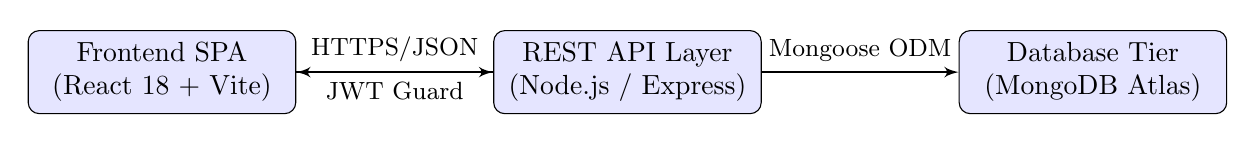
\begin{tikzpicture}[node distance=1.8cm, auto]
        \tikzstyle{block} = [rectangle, draw, fill=blue!10, text width=9em, text centered, rounded corners, minimum height=3em]
        \tikzstyle{line} = [draw, -latex', thick]

        \node [block] (ui) {Frontend SPA\\(React 18 + Vite)};
        \node [block, right=2.5cm of ui] (api) {REST API Layer\\(Node.js / Express)};
        \node [block, right=2.5cm of api] (db) {Database Tier\\(MongoDB Atlas)};

        \path [line] (ui) -- node[above]{\small HTTPS/JSON} (api);
        \path [line] (api) -- node[above]{\small Mongoose ODM} (db);
        \path [line] (api) -- node[below]{\small JWT Guard} (ui);
    \end{tikzpicture}
    \caption{Conceptual Three-Tier Application Architecture}
    \label{fig:tech_landscape}
\end{figure}

Figure~\ref{fig:tech_landscape} shows the three-tier architecture used in the project: a React single-page application, an Express/Node.js API layer, and a MongoDB database tier. I selected the MERN stack because it keeps both frontend and backend development in JavaScript, which was practical for a small internship project \cite{mern}. React supports reusable UI components for product cards, filters, forms, dashboards, and checkout screens \cite{react}. Express provides simple routing and middleware patterns for authentication, validation, and REST API endpoints \cite{express}. MongoDB supports flexible document structures, which is useful because product specifications vary across categories \cite{mongoose}.

Authentication and authorization were also important. JSON Web Tokens (JWTs) are commonly used for stateless authentication in REST APIs because the server can verify signed claims without keeping session state for every request \cite{jwt}. In this project, JWTs are combined with role-based middleware so customer routes and admin routes stay separate. Passwords are protected using bcrypt-style hashing, which is designed to be computationally expensive and adaptable as hardware improves \cite{bcrypt}. I also kept price calculation, stock decrement, and order status transitions on the server so they could not be changed from the browser.

\section{Competitive Analysis}
The competitive review suggests that Orient Computer should not try to compete only through visual design. Larger retailers already have product range, brand recognition, and online ordering. For this project, the more realistic goal was to build a maintainable system that fits Orient Computer's daily workflow. The platform includes customer-facing features such as search, cart persistence, checkout, order tracking, wishlist, and reviews, while also supporting staff-facing features such as inventory monitoring, order moderation, coupon control, dashboard analytics, and manual MFS payment verification.

This focus is important because Orient Computer's problem is not limited to publishing products online. The business also needs to turn browsing into verified orders, handle district-based delivery costs, manage stock changes, and review customer-submitted mobile payment evidence. The literature and market review therefore support three design priorities for the project: a familiar e-commerce interface for customers, a secure API and database foundation, and an admin panel that matches the real workflow of a Bangladeshi electronics retailer.

% ---------------------------------------------------------
% CHAPTER 3: PROJECT MANAGEMENT & FINANCING
% ---------------------------------------------------------
\chapter{Project Management and Financing}

\section{Work Breakdown Structure}
I organized the project into six main phases. Figure~\ref{fig:wbs} shows how the work was divided.

\begin{figure}[H]
    \centering
    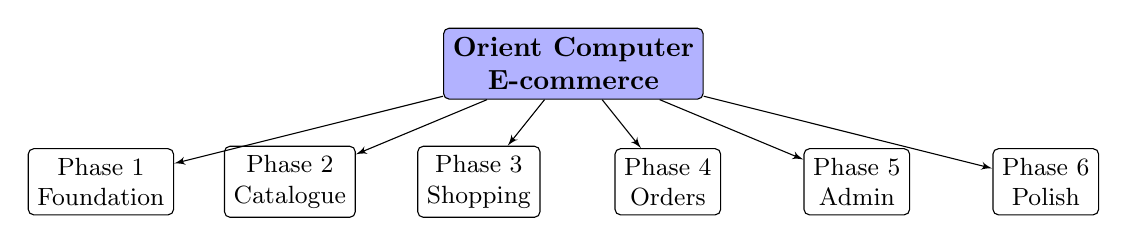
\begin{tikzpicture}[
        every node/.style={draw, rounded corners=2pt, font=\small, align=center},
        level 1/.style={sibling distance=2.4cm, fill=blue!15},
        edge from parent/.style={draw, -latex'}
    ]
    \node[fill=blue!30, font=\bfseries] {Orient Computer\\E-commerce}
        child {node {Phase 1\\Foundation}}
        child {node {Phase 2\\Catalogue}}
        child {node {Phase 3\\Shopping}}
        child {node {Phase 4\\Orders}}
        child {node {Phase 5\\Admin}}
        child {node {Phase 6\\Polish}};
    \end{tikzpicture}
    \caption{Work Breakdown Structure (WBS) Diagram}
    \label{fig:wbs}
\end{figure}

\section{Process and Activity Time Distribution}
Table~\ref{tab:time_distribution} outlines the estimated versus actual timeline allocated to each project phase over the 13-week development period.

\begin{table}[H]
\centering
\caption{Time Distribution by Project Phase}
\label{tab:time_distribution}
\begin{tabularx}{0.85\textwidth}{Xcc}
\toprule
\textbf{Phase Description} & \textbf{Estimated (Days)} & \textbf{Actual (Days)} \\
\midrule
Phase 1: Foundation (Setup, Auth, Base UI) & 10 & 12 \\
Phase 2: Catalogue (Categories, Products, Search) & 14 & 16 \\
Phase 3: Shopping (Cart, Checkout, Payments) & 12 & 15 \\
Phase 4: Orders (Creation, Tracking, Lifecycle) & 10 & 11 \\
Phase 5: Admin Panel (Management Dashboard) & 16 & 18 \\
Phase 6: Extras and Final Polish & 8 & 10 \\
\midrule
\textbf{Total Project Duration} & \textbf{70} & \textbf{82} \\
\bottomrule
\end{tabularx}
\end{table}

\section{Gantt Chart}
Figure~\ref{fig:gantt} shows the project timeline and the overlap between different phases.

\begin{figure}[H]
\centering
\begin{ganttchart}[
    vgrid,
    hgrid,
    x unit=0.9cm,
    y unit chart=0.6cm,
    time slot format=simple,
    bar/.append style={fill=blue!40},
    bar height=0.5
]{1}{13}
\gantttitle{Project Schedule (13 Weeks)}{13} \\
\gantttitlelist{1,...,13}{1} \\
\ganttbar{Phase 1: Foundation}{1}{2} \\
\ganttbar{Phase 2: Catalogue}{3}{5} \\
\ganttbar{Phase 3: Shopping}{5}{7} \\
\ganttbar{Phase 4: Orders}{7}{9} \\
\ganttbar{Phase 5: Admin}{9}{12} \\
\ganttbar{Phase 6: Polish}{11}{13}
\end{ganttchart}
\caption{Project Gantt Chart}
\label{fig:gantt}
\end{figure}

\section{Resource Allocation and Estimated Costing}
Hardware and infrastructure resources were carefully managed to minimize overhead during development.

\begin{table}[H]
\centering
\caption{Estimated Project Development and Hosting Cost}
\label{tab:costing}
\begin{tabularx}{0.9\textwidth}{Xr}
\toprule
\textbf{Item Description} & \textbf{Estimated Cost (BDT)} \\
\midrule
Development Workstation (Existing Core i7, 16GB RAM) & 0 \\
Database Hosting (MongoDB Atlas M0 Free Cluster) & 0 \\
Development Software \& Tooling (VS Code, Git, Postman) & 0 \\
Domain Registration (Annual .com/.com.bd) & $\sim 1{,}500$ \\
Frontend Hosting (Vercel Production Edge CDN) & 0 \\
Backend API Hosting (Railway/Render Container Instance) & $\sim 1{,}200$ / month \\
Internet and Connectivity (3 Months Development) & $\sim 3{,}000$ \\
\midrule
\textbf{Total Setup Cost (Excluding Recurring Cloud Hosting)} & \textbf{$\sim 4{,}500$ BDT} \\
\bottomrule
\end{tabularx}
\end{table}

% ---------------------------------------------------------
% CHAPTER 4: METHODOLOGY
% ---------------------------------------------------------
\chapter{Methodology}

\section{Architecture Overview}
The application uses a three-tier client-server architecture. The browser communicates with the Node.js/Express backend through REST API endpoints. The backend handles validation and then communicates with MongoDB Atlas through Mongoose schemas. Figure~\ref{fig:detailed_arch} shows how the main components communicate with each other.

\begin{figure}[H]
\centering
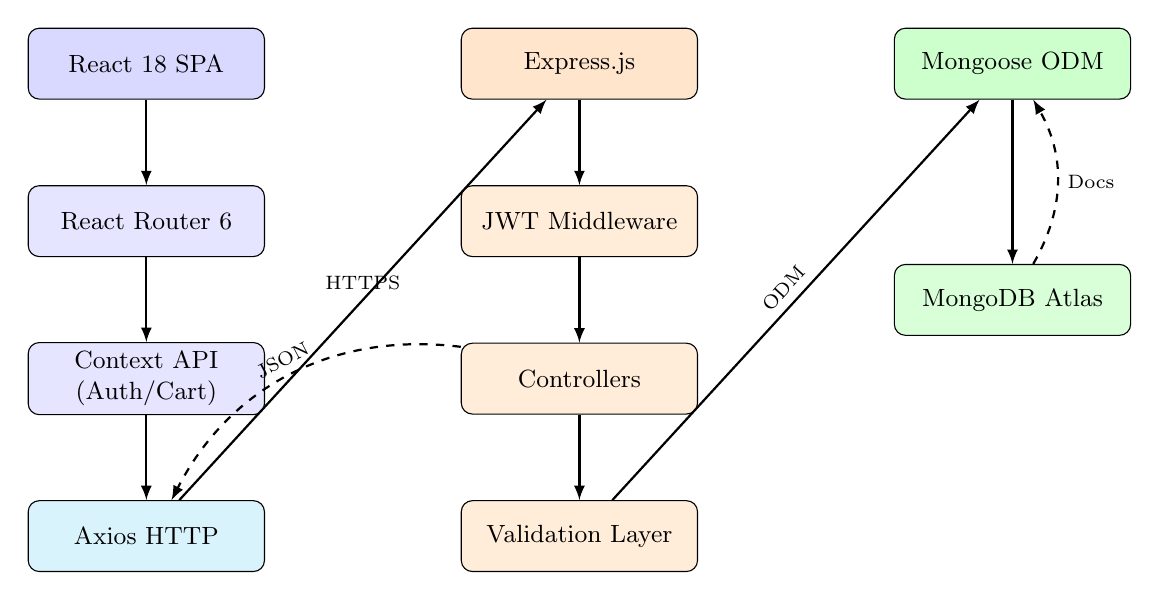
\begin{tikzpicture}[
    box/.style={draw, rounded corners=4pt, fill=#1, minimum width=3.0cm, minimum height=0.9cm, align=center, font=\small},
    arr/.style={-{latex}, thick},
    dasharr/.style={-{latex}, thick, dashed}
]
    % Client column
    \node[box=blue!15] (react)  at (0,0)    {React 18 SPA};
    \node[box=blue!10] (router) at (0,-2)   {React Router 6};
    \node[box=blue!10] (ctx)    at (0,-4)   {Context API\\(Auth/Cart)};
    \node[box=cyan!15] (axios)  at (0,-6)   {Axios HTTP};

    % Server column
    \node[box=orange!20] (express) at (5.5,0)  {Express.js};
    \node[box=orange!15] (auth)    at (5.5,-2) {JWT Middleware};
    \node[box=orange!15] (ctrl)    at (5.5,-4) {Controllers};
    \node[box=orange!15] (valid)   at (5.5,-6) {Validation Layer};

    % DB column
    \node[box=green!20] (mongoose) at (11,0)   {Mongoose ODM};
    \node[box=green!15] (atlas)    at (11,-3)  {MongoDB Atlas};

    % Request flow
    \draw[arr] (axios)   -- node[above,font=\scriptsize]{HTTPS} (express);
    \draw[arr] (express) -- (auth);
    \draw[arr] (auth)    -- (ctrl);
    \draw[arr] (ctrl)    -- (valid);
    \draw[arr] (valid)   -- node[above,font=\scriptsize,sloped]{ODM} (mongoose);
    \draw[arr] (mongoose) -- (atlas);

    % Internal client
    \draw[arr] (react)  -- (router);
    \draw[arr] (router) -- (ctx);
    \draw[arr] (ctx)    -- (axios);

    % Response arrows
    \draw[dasharr, bend right=30] (atlas) to node[right,font=\scriptsize]{Docs} (mongoose);
    \draw[dasharr, bend right=35] (ctrl)  to node[above,font=\scriptsize,sloped]{JSON} (axios);
\end{tikzpicture}
\caption{Detailed Component Architecture and Request/Response Flow}
\label{fig:detailed_arch}
\end{figure}

\section{Technology Stack}
Table~\ref{tab:tech_stack} lists the main libraries and tools used in the project.

\begin{table}[H]
\centering
\caption{Technology Stack}
\label{tab:tech_stack}
\begin{tabularx}{\textwidth}{lp{4cm}X}
\toprule
\textbf{Layer} & \textbf{Technology} & \textbf{Rationale \& Purpose} \\
\midrule
Frontend & React 18 with Vite & Component-based UI development and fast local development builds. \\
Routing & React Router 6 & Declarative client-side routing with nested layout support. \\
Styling & Tailwind CSS 3 & Utility-first styling for responsive layouts. \\
State \& API & Context API + Axios & Shared auth/cart state and reusable HTTP request handling. \\
Backend & Node.js + Express.js & API routing, middleware, and backend business logic. \\
Database & MongoDB Atlas & Flexible schema support for different electronic product specifications. \\
Security & JWT + bcryptjs & Stateless authorization tokens and salted password hashing. \\
Sanitization & Helmet, Mongo-Sanitize & HTTP security headers and NoSQL query injection prevention. \\
\bottomrule
\end{tabularx}
\end{table}

\section{Database Design and API Structure}
Orders store point-in-time snapshots of purchased product data, such as title, unit price, and SKU. This means old orders remain accurate even if a product title, price, or catalogue entry is changed later.

\begin{table}[H]
\centering
\caption{Selected Core REST API Endpoints}
\label{tab:api_endpoints}
\begin{tabularx}{\textwidth}{llX}
\toprule
\textbf{Method} & \textbf{Endpoint Path} & \textbf{Description / Operation} \\
\midrule
\texttt{POST} & \texttt{/api/auth/register} & Register new customer account \\
\texttt{POST} & \texttt{/api/auth/login} & Authenticate credentials and return signed JWT \\
\texttt{GET}  & \texttt{/api/products} & Query catalog with filtering, sorting, and pagination \\
\texttt{GET}  & \texttt{/api/products/:id} & Retrieve single product details with reviews \\
\texttt{POST} & \texttt{/api/orders} & Create verified order with stock validation \\
\texttt{POST} & \texttt{/api/orders/track} & Public anonymous order tracking by number \& phone \\
\texttt{GET}  & \texttt{/api/admin/dashboard} & Fetch aggregate operational KPIs and recent orders \\
\texttt{PATCH} & \texttt{/api/admin/orders/:id/status} & Advance order lifecycle state with timeline logging \\
\texttt{PATCH} & \texttt{/api/admin/orders/:id/payment} & Approve or reject manual MFS transaction \\
\bottomrule
\end{tabularx}
\end{table}

% ---------------------------------------------------------
% CHAPTER 5: BODY OF THE PROJECT
% ---------------------------------------------------------
\chapter{Body of the Project}

\section{Work Description}
The main implementation work covered frontend components, Express controller logic, database schema design, and deployment preparation. One of the most important parts was the checkout flow, because it needed to create orders, reduce stock correctly, and keep the order status consistent.

\section{Requirement Analysis}
Figure~\ref{fig:rich_picture} shows the system rich picture, including the main users, admin staff, and system components.

\begin{figure}[H]
\centering
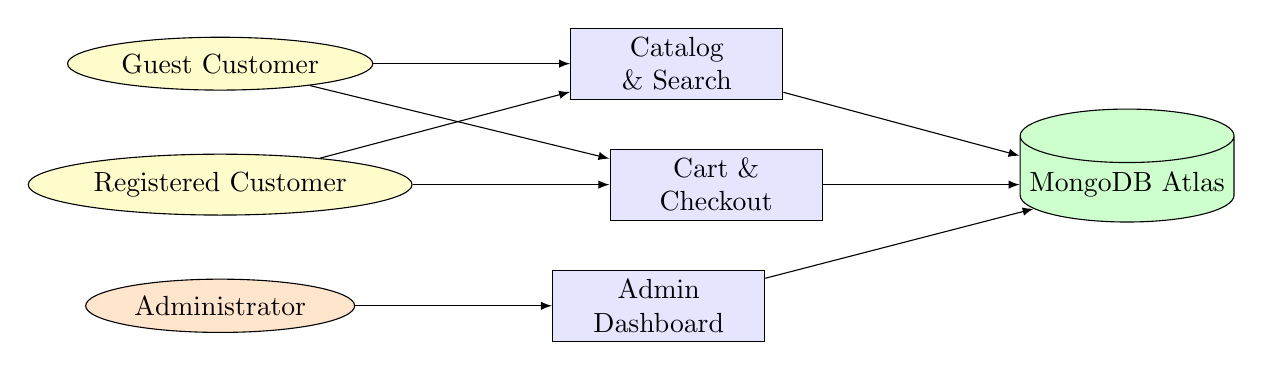
\begin{tikzpicture}[node distance=1.5cm, auto, >=latex]
    \node [draw, ellipse, fill=yellow!20] (guest) {Guest Customer};
    \node [draw, ellipse, fill=yellow!20, below=0.8cm of guest] (user) {Registered Customer};
    \node [draw, ellipse, fill=orange!20, below=0.8cm of user] (admin) {Administrator};

    \node [draw, rectangle, fill=blue!10, text width=7em, text centered, right=2.5cm of guest] (catalog) {Catalog \& Search};
    \node [draw, rectangle, fill=blue!10, text width=7em, text centered, right=2.5cm of user] (cart) {Cart \& Checkout};
    \node [draw, rectangle, fill=blue!10, text width=7em, text centered, right=2.5cm of admin] (adminp) {Admin Dashboard};

    \node [draw, cylinder, shape border rotate=90, aspect=0.25, fill=green!20, right=2.5cm of cart] (db) {MongoDB Atlas};

    \draw [->] (guest) -- (catalog);
    \draw [->] (guest) -- (cart);
    \draw [->] (user)  -- (catalog);
    \draw [->] (user)  -- (cart);
    \draw [->] (admin) -- (adminp);
    \draw [->] (catalog) -- (db);
    \draw [->] (cart)    -- (db);
    \draw [->] (adminp)  -- (db);
\end{tikzpicture}
\caption{Rich Picture of Orient Computer E-commerce Platform}
\label{fig:rich_picture}
\end{figure}

\subsection{Functional Requirements}
The application satisfies the following core functional requirements:
\begin{enumerate}
    \item Customer account registration, login, and JWT-authenticated session persistence.
    \item Hierarchical catalog browsing with dynamic filtering by category, brand, and price.
    \item Technical specification displays tailored to diverse equipment categories.
    \item Client-side guest cart storage with automatic synchronization upon account login.
    \item Server-enforced checkout calculations with district-specific delivery charges.
    \item Support for COD and manual MFS payments (bKash/Nagad) with screenshot upload.
    \item Secure order tracking accessible via order reference and contact number.
    \item Full administrative control over inventory, catalog taxonomy, coupons, and orders.
    \item Controlled order status machine (Pending $\rightarrow$ Confirmed $\rightarrow$ Processing $\rightarrow$ Shipped $\rightarrow$ Delivered).
\end{enumerate}

\subsection{Non-Functional Requirements}
\begin{enumerate}
    \item \textbf{Responsiveness:} Fully adaptive layouts across mobile, tablet, and desktop screens.
    \item \textbf{Localization:} Currency representations in Bangladeshi Taka (Tk.) and validation of Bangladeshi mobile phone formats (\texttt{01XXXXXXXXX}).
    \item \textbf{Performance:} Page load completion within 3 seconds over 4G connections.
    \item \textbf{Security:} Passwords hashed with bcrypt (cost factor 10); sensitive internal error traces omitted from production responses.
\end{enumerate}

\section{System Analysis and Feasibility}
The project was technically feasible because React, Node.js, and MongoDB all have mature ecosystems and strong community support. It was also operationally feasible because the admin interface follows the existing showroom fulfillment process instead of forcing staff to learn a completely different workflow. Financially, the project is reasonable because the required cloud hosting cost is low compared with the value of automating product, order, and payment management.

\section{System Design and Data Modeling}
Figure~\ref{fig:erd} shows the entity relationship model for the database collections.

\begin{figure}[H]
\centering
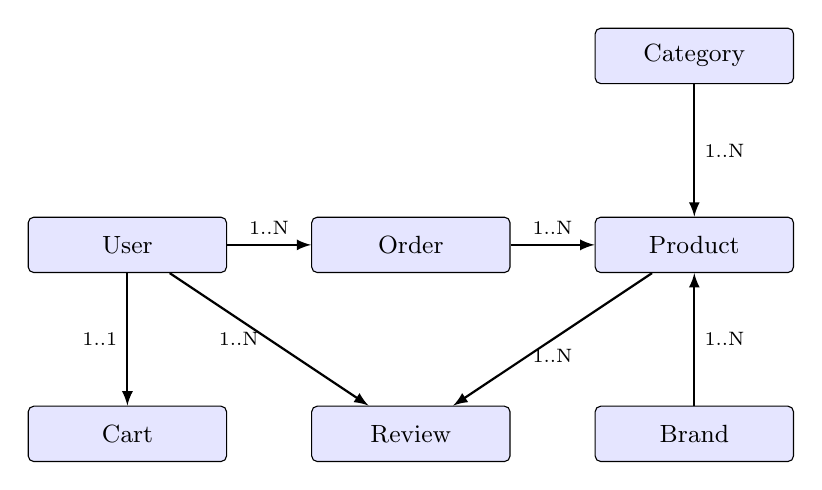
\begin{tikzpicture}[
    entity/.style={draw, rectangle, fill=blue!10, text width=6.5em, text centered, minimum height=2em, rounded corners=2pt, font=\small},
    rel/.style={draw, -latex, thick}
]
    \node[entity] (user)     at (0,0)    {User};
    \node[entity] (order)    at (3.6,0)  {Order};
    \node[entity] (product)  at (7.2,0)  {Product};
    \node[entity] (category) at (7.2,2.4){Category};
    \node[entity] (brand)    at (7.2,-2.4){Brand};
    \node[entity] (cart)     at (0,-2.4) {Cart};
    \node[entity] (review)   at (3.6,-2.4){Review};

    \draw[rel] (user)     -- node[above]{\scriptsize 1..N} (order);
    \draw[rel] (user)     -- node[left]{\scriptsize 1..1} (cart);
    \draw[rel] (category) -- node[right]{\scriptsize 1..N} (product);
    \draw[rel] (brand)    -- node[right]{\scriptsize 1..N} (product);
    \draw[rel] (order)    -- node[above]{\scriptsize 1..N} (product);
    \draw[rel] (user)     -- node[left]{\scriptsize 1..N} (review);
    \draw[rel] (product)  -- node[below]{\scriptsize 1..N} (review);
\end{tikzpicture}
\caption{Entity Relationship Diagram (ERD)}
\label{fig:erd}
\end{figure}

\subsection{MongoDB Collection Schema Summary}
\begin{table}[H]
\centering
\caption{MongoDB Collection Schema Summary}
\label{tab:schemas}
\begin{tabularx}{\textwidth}{lX}
\toprule
\textbf{Collection} & \textbf{Key Fields} \\
\midrule
\texttt{users} & name, email, password (bcrypt), role, phone, address \{division, district, street\}, avatar \\
\texttt{products} & title, slug, brand, category (ref), price, discountPrice, stock, sku, images[], shortSpecs[], technicalSpecs (Map), reviews[], isFeatured, badge \\
\texttt{categories} & name, slug, parent (self-ref), image, isActive \\
\texttt{orders} & user (ref), orderItems[], shippingAddress, paymentMethod, paymentResult, itemsPrice, shippingPrice, totalPrice, isPaid, orderStatus, trackingNumber, statusHistory[] \\
\texttt{coupons} & code, discountType, discountValue, minOrderValue, maxUses, validUntil, isActive \\
\texttt{carts} & user (ref), items[] \{product, qty, price\} \\
\bottomrule
\end{tabularx}
\end{table}

\section{UI Page Mockups}

The following figures show screenshots from the completed application. I added a short description under each screenshot to explain the purpose of the screen and the main visible features.

% --- Homepage Screenshot ---
\begin{figure}[H]
\centering
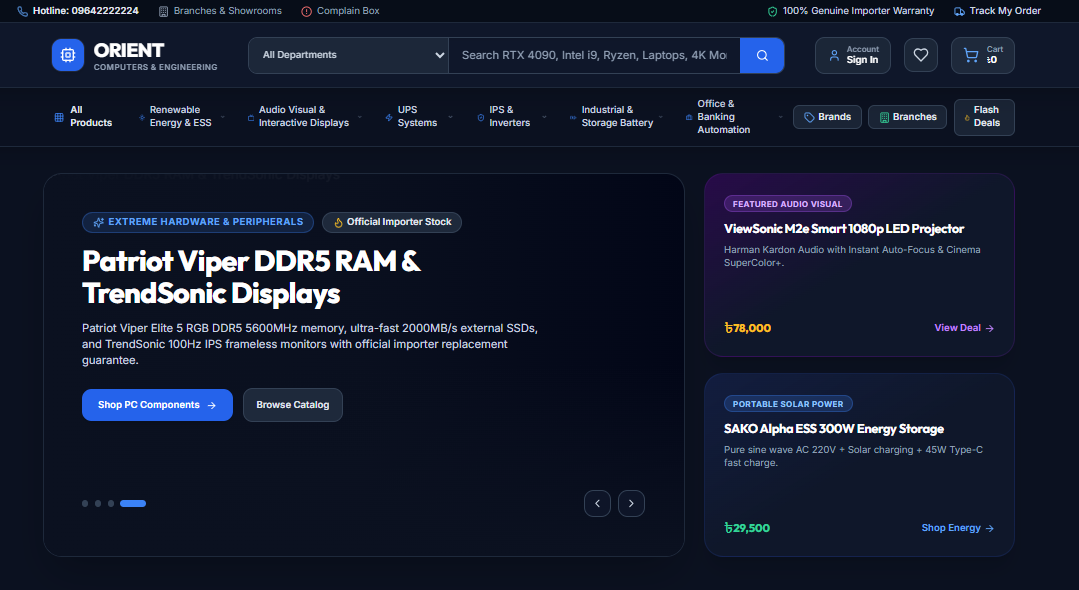
\includegraphics[width=\textwidth]{homePage.PNG}
\par\vspace{0.35cm}
\refstepcounter{figure}\small\textbf{Figure \thefigure: Homepage Screenshot}\\
\textbf{Description:} The homepage screenshot shows the public entry point of the Orient Computer e-commerce platform. It highlights the navigation bar, search access, promotional banner, featured product sections, and product cards that guide customers toward browsing and purchasing computer, power backup, and accessory products.
\label{fig:mockup_home}
\end{figure}

% --- Shop Page Screenshot ---
\begin{figure}[H]
\centering
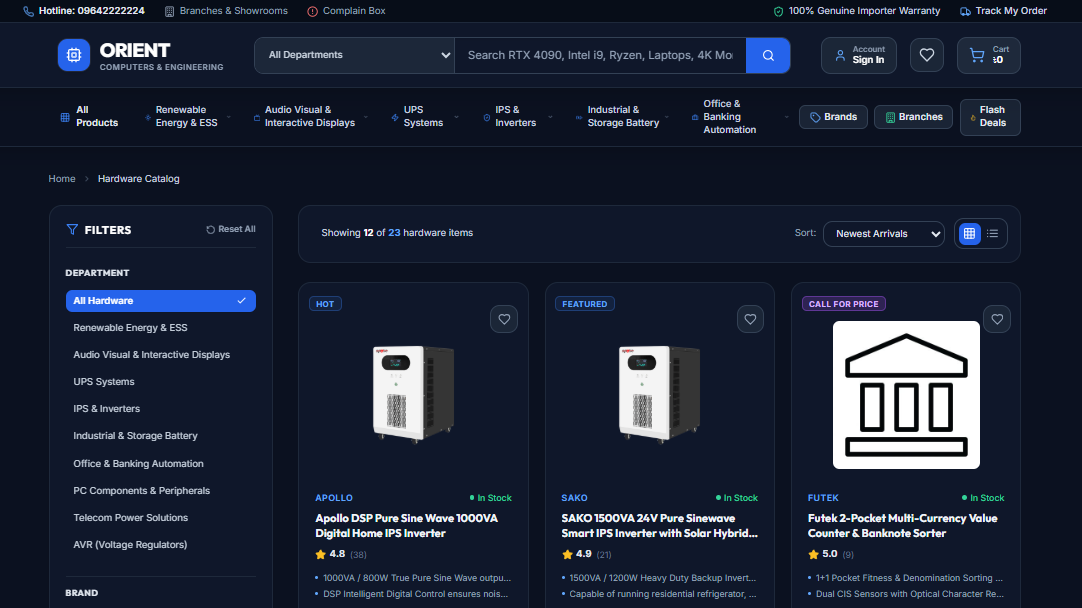
\includegraphics[width=\textwidth]{shopCatalogPage.PNG}
\par\vspace{0.35cm}
\refstepcounter{figure}\small\textbf{Figure \thefigure: Shop Catalog Screenshot}\\
\textbf{Description:} The shop catalog screenshot demonstrates the product browsing experience. It presents category and product discovery features, including filtering, sorting, product listings, prices, stock indicators, and add-to-cart actions that help customers compare items before purchase.
\label{fig:mockup_shop}
\end{figure}

% --- Product Detail Page Screenshot ---
\begin{figure}[H]
\centering
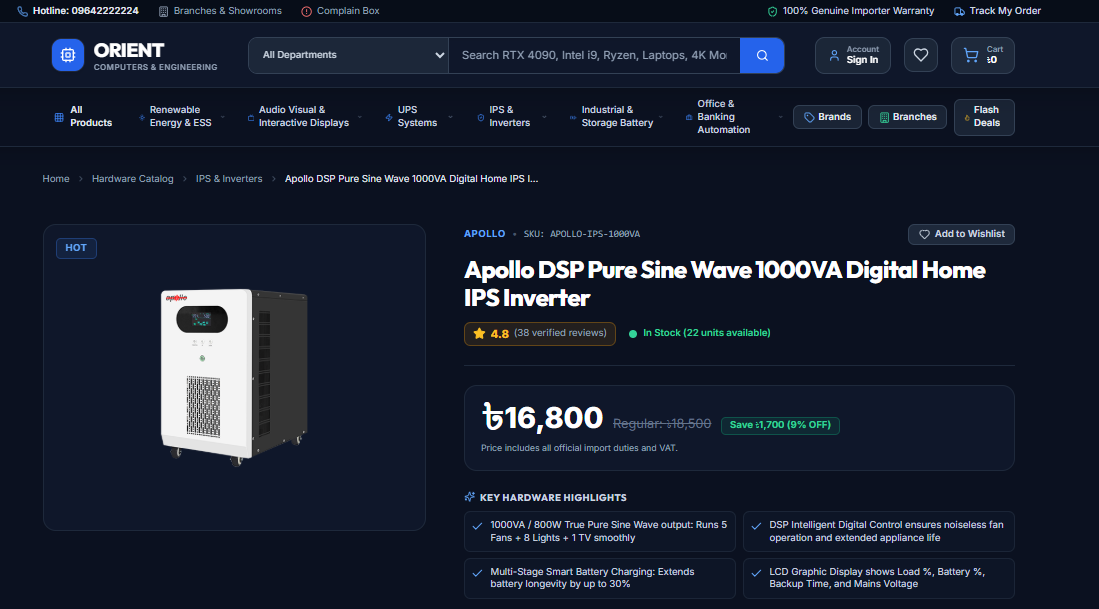
\includegraphics[width=\textwidth]{productDetailsPage.PNG}
\par\vspace{0.35cm}
\refstepcounter{figure}\small\textbf{Figure \thefigure: Product Detail Screenshot}\\
\textbf{Description:} The product detail screenshot displays the dedicated product information page. It shows the selected product image, pricing, availability, technical details, quantity selection, and purchase actions, allowing customers to evaluate a product before adding it to the cart or proceeding directly to checkout.
\label{fig:mockup_product}
\end{figure}

% --- Checkout Page Screenshot ---
\begin{figure}[H]
\centering
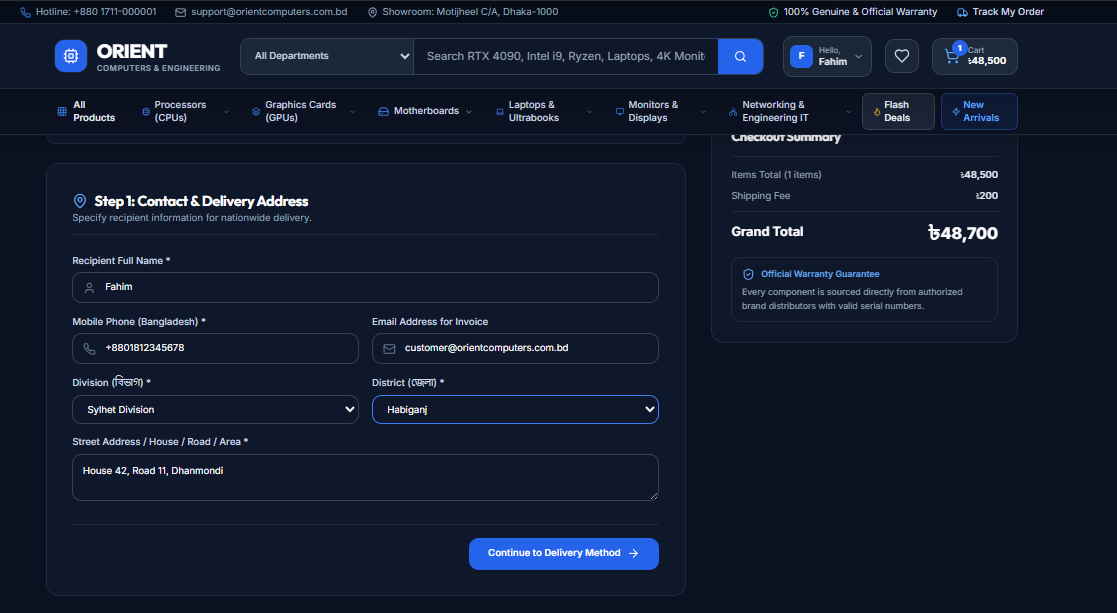
\includegraphics[width=\textwidth]{checkoutPage.PNG}
\par\vspace{0.35cm}
\refstepcounter{figure}\small\textbf{Figure \thefigure: Checkout Screenshot}\\
\textbf{Description:} The checkout screenshot illustrates the order completion workflow. It includes customer shipping information, order summary, payment method selection, coupon handling, and final order placement, supporting both cash-on-delivery and manual mobile financial service payment flows.
\label{fig:mockup_checkout}
\end{figure}

% --- Admin Dashboard Screenshot ---
\begin{figure}[H]
\centering
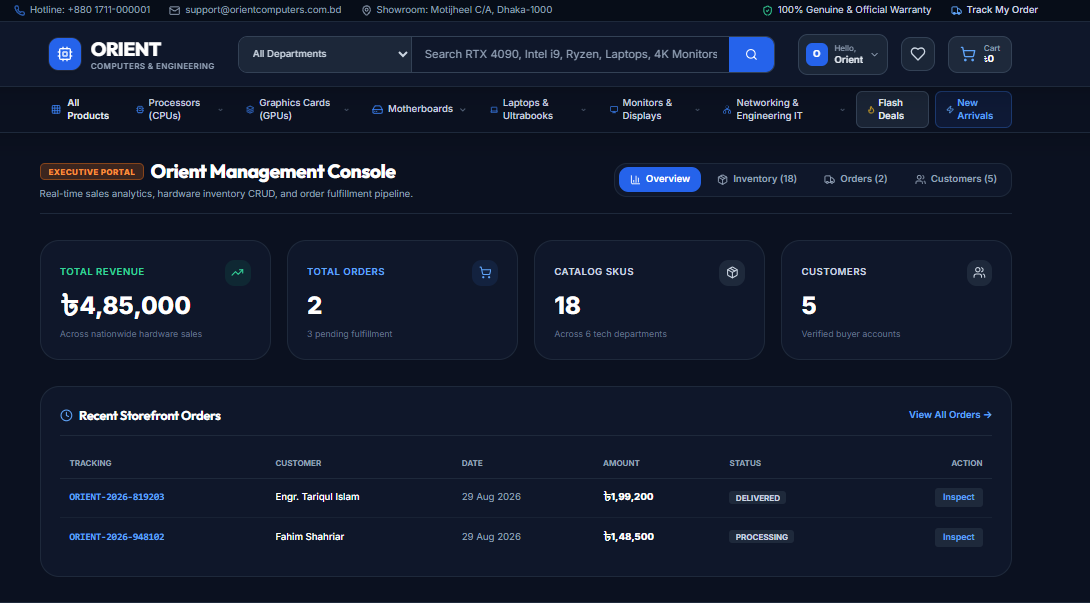
\includegraphics[width=\textwidth]{adminDashboard.PNG}
\par\vspace{0.35cm}
\refstepcounter{figure}\small\textbf{Figure \thefigure: Admin Dashboard Screenshot}\\
\textbf{Description:} The admin dashboard screenshot shows the management overview for store administrators. It summarizes key operational metrics such as revenue, orders, users, and products, while also giving quick access to charts and recent activity for monitoring business performance.
\label{fig:mockup_admin}
\end{figure}

% --- Admin Orders Screenshot ---
\begin{figure}[H]
\centering
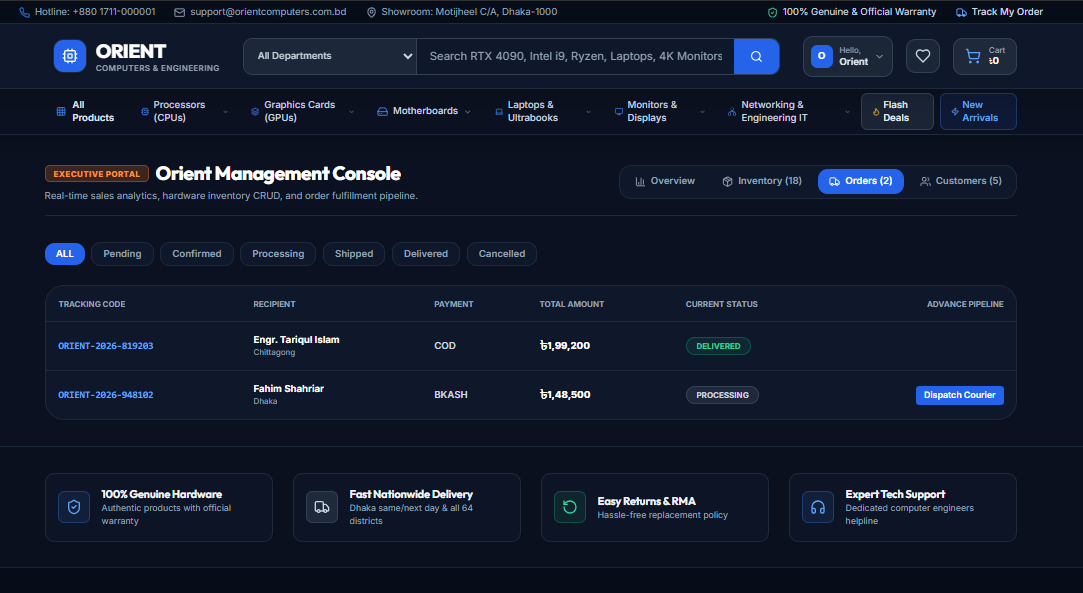
\includegraphics[width=\textwidth]{adminDashboardOrders.PNG}
\par\vspace{0.35cm}
\refstepcounter{figure}\small\textbf{Figure \thefigure: Admin Orders Screenshot}\\
\textbf{Description:} The admin orders screenshot presents the order management interface. Administrators can review order records, inspect customer and payment details, track fulfillment status, and verify manually submitted payment screenshots before approving or updating an order.
\label{fig:mockup_admin_orders}
\end{figure}

% --- Admin Inventory Screenshot ---
\begin{figure}[H]
\centering
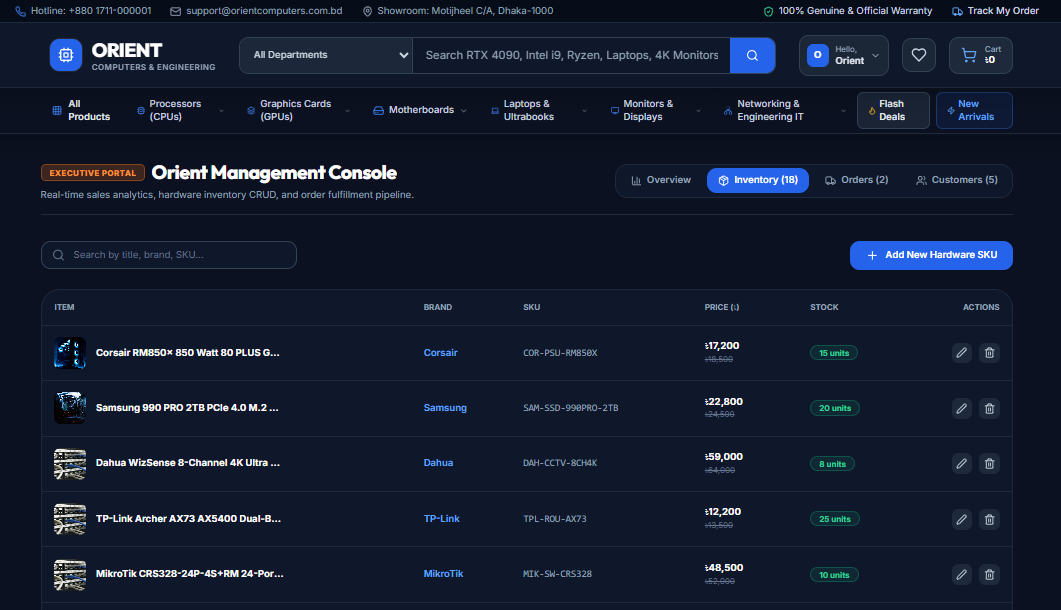
\includegraphics[width=\textwidth]{adminDashboardInventory.PNG}
\par\vspace{0.35cm}
\refstepcounter{figure}\small\textbf{Figure \thefigure: Admin Inventory Screenshot}\\
\textbf{Description:} The admin inventory screenshot shows the product and stock management area. It helps administrators monitor available products, identify low-stock items, update product information, and keep the catalog aligned with current store inventory.
\label{fig:mockup_admin_inventory}
\end{figure}

% --- Admin Customers Screenshot ---
\begin{figure}[H]
\centering
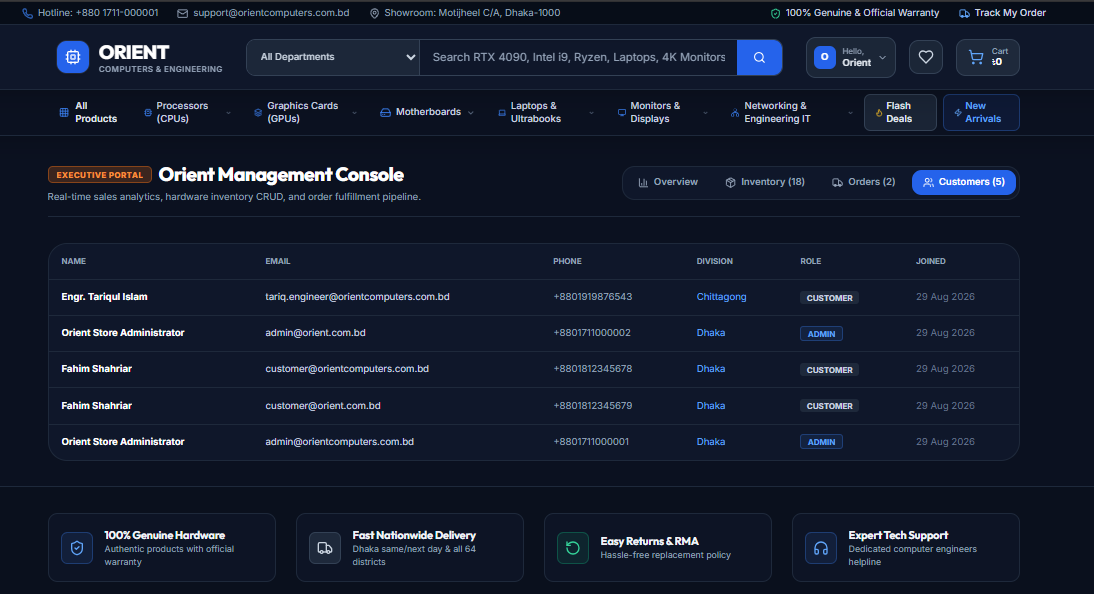
\includegraphics[width=\textwidth]{adminDashboardCustomers.PNG}
\par\vspace{0.35cm}
\refstepcounter{figure}\small\textbf{Figure \thefigure: Admin Customers Screenshot}\\
\textbf{Description:} The admin customers screenshot displays the customer management view. It provides administrators with an overview of registered users, customer contact information, account roles, and related activity useful for support and order follow-up.
\label{fig:mockup_admin_customers}
\end{figure}

\section{Order State Machine}
Figure~\ref{fig:state_machine} shows the finite-state machine used for order status changes on the server.

\begin{figure}[H]
\centering
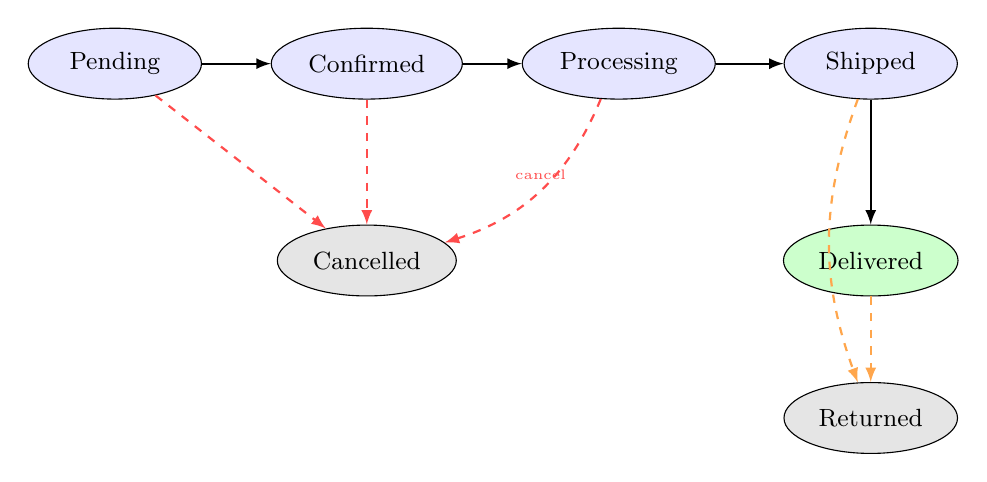
\begin{tikzpicture}[
    state/.style={draw, ellipse, fill=blue!10, minimum width=2.2cm, minimum height=0.9cm, align=center, font=\small},
    terminal/.style={draw, ellipse, fill=gray!20, minimum width=2.2cm, minimum height=0.9cm, align=center, font=\small},
    arr/.style={-{latex}, thick}
]
    \node[state] (pending)    at (0,0)    {Pending};
    \node[state] (confirmed)  at (3.2,0)  {Confirmed};
    \node[state] (processing) at (6.4,0)  {Processing};
    \node[state] (shipped)    at (9.6,0)  {Shipped};
    \node[state, fill=green!20] (delivered) at (9.6,-2.5) {Delivered};
    \node[terminal] (cancelled) at (3.2,-2.5) {Cancelled};
    \node[terminal] (returned)  at (9.6,-4.5) {Returned};

    \draw[arr] (pending)    -- (confirmed);
    \draw[arr] (confirmed)  -- (processing);
    \draw[arr] (processing) -- (shipped);
    \draw[arr] (shipped)    -- (delivered);

    \draw[arr, dashed, color=red!70] (pending)    -- (cancelled);
    \draw[arr, dashed, color=red!70] (confirmed)  -- (cancelled);
    \draw[arr, dashed, color=red!70] (processing) to[bend left=25] node[above,font=\tiny]{cancel} (cancelled);
    \draw[arr, dashed, color=orange!70] (shipped)   to[bend right=20] (returned);
    \draw[arr, dashed, color=orange!70] (delivered) -- (returned);
\end{tikzpicture}
\caption{Order Lifecycle Finite-State Machine}
\label{fig:state_machine}
\end{figure}

\begin{table}[H]
\centering
\caption{Permitted Order Status State Transitions}
\label{tab:status_transitions}
\begin{tabularx}{0.8\textwidth}{lX}
\toprule
\textbf{Current Status} & \textbf{Permitted Subsequent Statuses} \\
\midrule
Pending & Confirmed, Cancelled \\
Confirmed & Processing, Cancelled \\
Processing & Shipped, Cancelled \\
Shipped & Delivered, Returned \\
Delivered & Returned \\
Cancelled / Returned & (Terminal States -- None) \\
\bottomrule
\end{tabularx}
\end{table}

\section{Key Code Implementations}

\subsection{User Schema with bcrypt Password Hashing}

The \texttt{User} Mongoose schema enforces server-side password hashing using bcrypt before saving to the database, preventing plain-text credential exposure. Listing~\ref{lst:user_model} shows the complete model.

\begin{lstlisting}[language=JavaScript, caption={User.js -- Mongoose Schema with bcrypt Pre-Save Hook}, label={lst:user_model}]
import mongoose from 'mongoose';
import bcrypt from 'bcryptjs';

const userSchema = new mongoose.Schema({
  name:  { type: String, required: true, trim: true, maxlength: 50 },
  email: {
    type: String, required: true, unique: true, lowercase: true,
    match: [/^\w+([.-]?\w+)*@\w+([.-]?\w+)*(\.\w{2,3})+$/,
            'Please provide a valid email'],
  },
  password: {
    type: String, required: true, minlength: 6,
    select: false,  // excluded from queries by default
  },
  role:   { type: String, enum: ['customer','admin'], default: 'customer' },
  phone:  { type: String, default: '' },
  avatar: { type: String, default: '' },
  address: {
    division:   { type: String, default: 'Dhaka'       },
    district:   { type: String, default: 'Dhaka'       },
    street:     { type: String, default: ''             },
    postalCode: { type: String, default: ''             },
    country:    { type: String, default: 'Bangladesh'   },
  },
}, { timestamps: true });

// Hash password before saving if modified
userSchema.pre('save', async function (next) {
  if (!this.isModified('password')) return next();
  const salt = await bcrypt.genSalt(10);
  this.password = await bcrypt.hash(this.password, salt);
  next();
});

// Instance method for login password comparison
userSchema.methods.matchPassword = async function (entered) {
  return await bcrypt.compare(entered, this.password);
};

export default mongoose.model('User', userSchema);
\end{lstlisting}

\subsection{JWT Authentication Middleware}

Listing~\ref{lst:auth_middleware} presents the three-tier middleware chain: mandatory \texttt{protect}, guest-tolerant \texttt{optionalProtect}, and \texttt{admin} privilege guard.

\begin{lstlisting}[language=JavaScript, caption={authMiddleware.js -- JWT Protection and Admin Guard}, label={lst:auth_middleware}]
import jwt from 'jsonwebtoken';
import User from '../models/User.js';

// Mandatory JWT authentication
export const protect = async (req, res, next) => {
  let token;
  if (req.headers.authorization?.startsWith('Bearer')) {
    try {
      token = req.headers.authorization.split(' ')[1];
      const decoded = jwt.verify(token,
        process.env.JWT_SECRET || 'orient_jwt_secret_key_2026'
      );
      const user = await User.findById(decoded.id).select('-password');
      if (!user) {
        res.status(401);
        return next(new Error('User not found. Authorization failed.'));
      }
      req.user = user;
      return next();
    } catch {
      res.status(401);
      return next(new Error('Invalid or expired token. Not authorized.'));
    }
  }
  res.status(401);
  return next(new Error('No token provided. Not authorized.'));
};

// Optional: populates req.user if token present, allows guests otherwise
export const optionalProtect = async (req, res, next) => {
  if (req.headers.authorization?.startsWith('Bearer')) {
    try {
      const token = req.headers.authorization.split(' ')[1];
      const decoded = jwt.verify(token,
        process.env.JWT_SECRET || 'orient_jwt_secret_key_2026'
      );
      const user = await User.findById(decoded.id).select('-password');
      if (user) req.user = user;
    } catch { req.user = null; }
  }
  return next();
};

// Administrator privilege guard
export const admin = (req, res, next) => {
  if (req.user?.role === 'admin') return next();
  res.status(403);
  return next(new Error('Access denied. Administrator privileges required.'));
};
\end{lstlisting}

\subsection{Product Schema with Virtuals and Text Index}

Listing~\ref{lst:product_model} demonstrates the \texttt{Product} schema with a \texttt{Map}-typed \texttt{technicalSpecs} field for flexible hardware specifications, computed virtuals for stock status and discount percentage, and a compound text index for full-text catalog search.

\begin{lstlisting}[language=JavaScript, caption={Product.js -- Schema with Virtuals and Full-Text Index}, label={lst:product_model}]
const productSchema = new mongoose.Schema({
  title:         { type: String, required: true, trim: true },
  slug:          { type: String, required: true, unique: true, lowercase: true },
  brand:         { type: String, required: true },
  category:      { type: mongoose.Schema.Types.ObjectId,
                   ref: 'Category', required: true },
  price:         { type: Number, required: true, min: 0 },
  discountPrice: { type: Number, default: 0 },
  stock:         { type: Number, required: true, min: 0, default: 0 },
  sku:           { type: String, required: true, unique: true, uppercase: true },
  images:        { type: [String], required: true },
  shortSpecs:    { type: [String], default: [] },
  // Flexible key-value map for diverse hardware spec sheets
  technicalSpecs:{ type: Map, of: String, default: {} },
  warranty:      { type: String, default: 'Official Brand Warranty' },
  reviews:       [reviewSchema],
  isFeatured:    { type: Boolean, default: false },
  badge: {
    type: String,
    enum: ['', 'HOT', 'SALE', 'NEW', 'GAMING', 'OFFER', 'FEATURED'],
    default: '',
  },
}, { timestamps: true, toJSON: { virtuals: true } });

// Virtual: inStock computed from stock quantity
productSchema.virtual('inStock').get(function () {
  return this.stock > 0;
});

// Virtual: discount percentage calculation
productSchema.virtual('discountPercentage').get(function () {
  if (this.discountPrice && this.discountPrice < this.price)
    return Math.round(((this.price - this.discountPrice) / this.price) * 100);
  return 0;
});

// Compound text index for full-text catalog search
productSchema.index({
  title: 'text', brand: 'text',
  shortSpecs: 'text', sku: 'text',
});
\end{lstlisting}

\subsection{Order Creation with Guest Checkout and Atomic Stock Decrement}

Listing~\ref{lst:order_create} shows the order creation controller. It supports both authenticated users and guests (by provisioning implicit accounts), performs atomic stock decrements per purchased SKU, and returns an auto-generated tracking number of the form \texttt{ORIENT-YYYY-XXXXXX}.

\begin{lstlisting}[language=JavaScript, caption={orderController.js -- createOrder with Guest Account Provisioning and Stock Decrement}, label={lst:order_create}]
export const createOrder = async (req, res, next) => {
  try {
    const { orderItems, shippingAddress, paymentMethod,
            itemsPrice, shippingPrice, discountPrice, totalPrice } = req.body;

    if (!orderItems?.length) {
      res.status(400);
      return next(new Error('No order items provided.'));
    }

    let orderUser = req.user;
    let autoCreatedToken = null;

    // Guest checkout: find existing user by phone/email or create one
    if (!orderUser) {
      const cleanPhone = (shippingAddress.phone || '').replace(/[^0-9+]/g, '');
      const guestEmail = (shippingAddress.email ||
        `guest_${cleanPhone || Date.now()}@orientcomputers.com.bd`).toLowerCase();

      let user = await User.findOne({
        $or: [{ email: guestEmail },
              ...(cleanPhone ? [{ phone: cleanPhone }] : [])],
      });

      if (!user) {
        const randomSecret = Math.random().toString(36).slice(-8);
        user = await User.create({
          name: shippingAddress.fullName,
          email: guestEmail,
          password: `Orient#${randomSecret}2026`,
          phone: cleanPhone || '',
          role: 'customer',
        });
      }
      orderUser = user;
      autoCreatedToken = generateToken(user._id);
    }

    const order = new Order({
      user: orderUser._id, orderItems, shippingAddress,
      paymentMethod, itemsPrice, shippingPrice, discountPrice, totalPrice,
      isPaid: paymentMethod !== 'COD',
      paidAt: paymentMethod !== 'COD' ? new Date() : null,
      orderStatus: 'Pending',
    });

    const createdOrder = await order.save();

    // Atomic stock decrement for each purchased SKU
    for (const item of orderItems) {
      if (item.product) {
        await Product.findByIdAndUpdate(item.product, {
          $inc: { stock: -Number(item.qty || 1) },
        });
      }
    }

    const payload = { success: true, order: createdOrder };
    if (autoCreatedToken) {
      payload.token = autoCreatedToken;
      payload.user  = { _id: orderUser._id, name: orderUser.name,
                        email: orderUser.email, role: orderUser.role };
    }
    res.status(201).json(payload);
  } catch (error) { next(error); }
};
\end{lstlisting}

\subsection{Admin Analytics Aggregation Pipeline}

Listing~\ref{lst:analytics} presents the dashboard analytics controller using MongoDB's aggregation framework with parallel \texttt{Promise.all} execution for optimal performance.

\begin{lstlisting}[language=JavaScript, caption={orderController.js -- Admin Dashboard Analytics with Aggregation Pipeline}, label={lst:analytics}]
export const getAdminAnalytics = async (req, res, next) => {
  try {
    // Run all count queries in parallel for performance
    const [totalOrders, pendingOrders, deliveredOrders,
           totalProducts, lowStockProducts, totalCustomers] =
      await Promise.all([
        Order.countDocuments({}),
        Order.countDocuments({ orderStatus: 'Pending' }),
        Order.countDocuments({ orderStatus: 'Delivered' }),
        Product.countDocuments({}),
        Product.countDocuments({ stock: { $lte: 5 } }),
        User.countDocuments({ role: 'customer' }),
      ]);

    // Aggregation pipeline: revenue excluding cancelled orders
    const revenueAgg = await Order.aggregate([
      { $match: { orderStatus: { $ne: 'Cancelled' } } },
      { $group: { _id: null, totalRevenue: { $sum: '$totalPrice' } } },
    ]);
    const totalRevenue = revenueAgg[0]?.totalRevenue || 0;

    const recentOrders = await Order.find({})
      .populate('user', 'name email')
      .sort({ createdAt: -1 })
      .limit(6);

    res.status(200).json({
      success: true,
      analytics: {
        totalRevenue, totalOrders, pendingOrders,
        deliveredOrders, totalProducts, lowStockProducts,
        totalCustomers, recentOrders,
      },
    });
  } catch (error) { next(error); }
};
\end{lstlisting}

\section{Implementation and Testing}
Testing covered the most important parts of the system: price and coupon calculations, API endpoints connected to MongoDB Atlas, and security checks for token manipulation and unauthorized admin access.

\begin{table}[H]
\centering
\caption{Key Test Case Summary}
\label{tab:test_cases}
\begin{tabularx}{\textwidth}{lXl}
\toprule
\textbf{Test ID} & \textbf{Test Scenario} & \textbf{Result} \\
\midrule
TC-01 & POST /api/auth/register with valid payload creates user and returns JWT & PASS \\
TC-02 & POST /api/auth/login with wrong password returns 401 Unauthorized & PASS \\
TC-03 & GET /api/products with category filter returns only matching products & PASS \\
TC-04 & POST /api/orders decrements stock atomically after successful creation & PASS \\
TC-05 & PATCH /api/admin/orders/:id/status without admin role returns 403 & PASS \\
TC-06 & Manipulated totalPrice in request body is ignored; server recalculates & PASS \\
TC-07 & Checkout with out-of-stock product returns 400 with descriptive error & PASS \\
TC-08 & Guest checkout creates implicit customer account and returns JWT & PASS \\
TC-09 & Invalid JWT token on protected route returns 401 Not Authorized & PASS \\
TC-10 & Order tracking by valid tracking number returns masked order details & PASS \\
\bottomrule
\end{tabularx}
\end{table}

% ---------------------------------------------------------
% CHAPTER 6: RESULTS AND ANALYSIS
% ---------------------------------------------------------
\chapter{Results and Analysis}

The Orient Computer platform was built and tested with realistic product data across 8 parent categories. I also checked the main pages on different screen sizes to make sure the customer and admin interfaces were usable.

\begin{table}[H]
\centering
\caption{System Performance and Latency Metrics}
\label{tab:latency_results}
\begin{tabularx}{\textwidth}{Xcr}
\toprule
\textbf{Transaction / Operation} & \textbf{Data Payload} & \textbf{Avg. Latency (ms)} \\
\midrule
Product Listing Query (filters \& pagination) & $\sim 24$ KB & 380 \\
Product Detail \& Specification Retrieval & $\sim 8$ KB & 220 \\
Order Creation (Validation, Price Freeze, DB Write) & $\sim 4$ KB & 740 \\
Admin Aggregate Dashboard KPI Calculation & $\sim 12$ KB & 450 \\
\bottomrule
\end{tabularx}
\end{table}

The benchmark results show that the main API responses stayed below the target limit of 3 seconds under realistic network conditions.

\section{System Features Delivered}
All five primary objectives defined in Chapter~1 were delivered:
\begin{itemize}
    \item \textbf{Customer Storefront:} Responsive React 18 SPA with 14 pages, dynamic catalog, and multi-step checkout.
    \item \textbf{Localized Payments:} COD, bKash, and Nagad workflows with payment proof submission and admin verification queue.
    \item \textbf{Admin Dashboard:} Operational KPI cards, order management table, low-stock alerts, and product/category CRUD.
    \item \textbf{Security:} bcrypt password hashing, JWT Bearer scheme, role-based guards, Helmet.js HTTP headers.
    \item \textbf{Guest Checkout:} Implicit account creation that allows checkout without prior registration.
\end{itemize}

\section{Deployment Architecture}
Figure~\ref{fig:deployment} illustrates the production deployment topology across cloud platforms.

\begin{figure}[H]
\centering
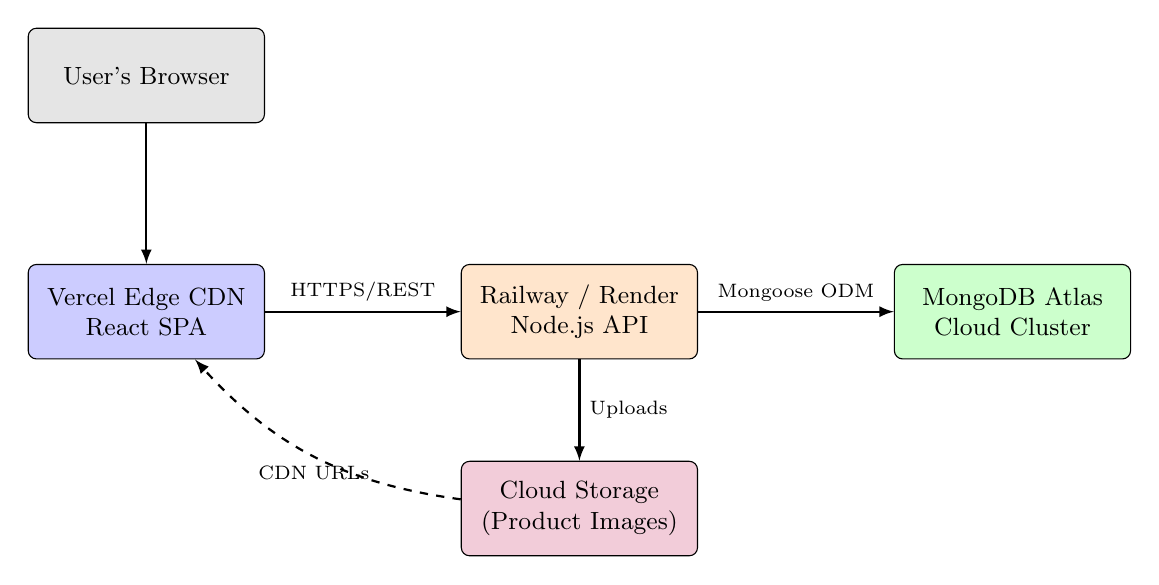
\begin{tikzpicture}[
    svc/.style={draw, rounded corners=3pt, fill=#1, minimum width=3cm, minimum height=1.2cm, align=center, font=\small},
    arr/.style={-{latex}, thick}
]
    \node[svc=gray!20]   (browser)   at (0,3)    {User's Browser};
    \node[svc=blue!20]   (vercel)    at (0,0)    {Vercel Edge CDN\\React SPA};
    \node[svc=orange!20] (server)    at (5.5,0)  {Railway / Render\\Node.js API};
    \node[svc=green!20]  (atlas)     at (11,0)   {MongoDB Atlas\\Cloud Cluster};
    \node[svc=purple!20] (cloud)     at (5.5,-2.5){Cloud Storage\\(Product Images)};

    \draw[arr] (browser) -- (vercel);
    \draw[arr] (vercel)  -- node[above]{\scriptsize HTTPS/REST} (server);
    \draw[arr] (server)  -- node[above]{\scriptsize Mongoose ODM} (atlas);
    \draw[arr] (server)  -- node[right]{\scriptsize Uploads} (cloud);
    \draw[arr, dashed] (cloud) to[bend left=20] node[below,font=\scriptsize]{CDN URLs} (vercel);
\end{tikzpicture}
\caption{Production Deployment Architecture}
\label{fig:deployment}
\end{figure}

% ---------------------------------------------------------
% CHAPTER 7: ENGINEERING PROBLEM ANALYSIS
% ---------------------------------------------------------
\chapter{Project as Engineering Problem Analysis}

\section{Sustainability of the Project}
The application codebase was organized with separation of concerns in mind. Database schemas, HTTP route controllers, middleware, and business logic were kept in separate files so the project would be easier to understand and extend later. The use of cloud hosting and MongoDB Atlas also reduces the need for maintaining dedicated physical infrastructure for a small business application.

\section{Social and Environmental Considerations}
By giving Orient Computer a digital storefront, customers from different districts in Bangladesh can check products and place orders without always visiting the showroom. This can reduce unnecessary travel for customers who only need product information or want to confirm availability before buying. The admin dashboard can also help staff become more comfortable with digital order and inventory management.

\section{Ethical and Legal Considerations}
Customer data is handled carefully in the system. Passwords are never stored in plain text, and payment screenshots submitted for MFS verification are available only to authorized administrators. The platform avoids collecting unnecessary analytics data beyond what is needed for normal operation.

% ---------------------------------------------------------
% CHAPTER 8: LESSONS LEARNED
% ---------------------------------------------------------
\chapter{Lessons Learned}

\section{Problems Faced}
\begin{itemize}
    \item \textbf{MongoDB Transactions on Standalone Instances:} Multi-document transactions require replica set configurations. During local testing, this caused issues, so I added fallback rollback logic for cases where transactions were not available.
    \item \textbf{Cart Synchronization Race Conditions:} Merging a guest cart from the browser with an existing server-side cart was more complicated than expected. I had to compare items one by one so product quantities and stock limits stayed correct.
    \item \textbf{Windows Path Separators in Multer:} File uploads produced backslash path separators on Windows. These had to be normalized into forward slashes so uploaded image URLs worked consistently.
    \item \textbf{District-wise Delivery Fee Complexity:} Bangladesh's 64 districts required a structured delivery fee setup. I first considered hard-coded values, but later moved the fee matrix into the database so admins could update it without changing code.
    \item \textbf{JWT Storage Security Trade-offs:} Storing JWTs in \texttt{localStorage} is simple, but it can expose tokens if an XSS attack occurs. For the current version, this risk is reduced through security headers and input sanitization. A future version should move authentication to \texttt{HttpOnly} cookies.
\end{itemize}

\section{Solutions and Retrospective Insights}
One lesson I learned is that shared business rules should be kept in one place. Moving price and coupon calculations into centralized service modules reduced duplicate code and made testing easier. I also learned that writing the SRS before implementation was useful because it clarified the expected features and reduced confusion during development. In future versions, tools such as Redis or TanStack React Query could improve caching and client-side data fetching.

% ---------------------------------------------------------
% CHAPTER 9: FUTURE WORK & CONCLUSION
% ---------------------------------------------------------
\chapter{Future Work and Conclusion}

\section{Future Work}
Planned enhancements include:
\begin{enumerate}
    \item Integrate automated payment gateways such as SSLCommerz or ShurjoPay to reduce the need for manual MFS screenshot verification.
    \item Add SMS and email notifications when order status changes.
    \item Build an interactive PC Builder tool with compatibility checking for DIY PC customers.
    \item Move authentication from localStorage JWT storage to CSRF-protected \texttt{HttpOnly} cookies for better protection against token theft.
    \item Add product recommendations based on order history and browsing behavior.
    \item Add Progressive Web App (PWA) support for offline browsing and home screen installation.
\end{enumerate}

\section{Conclusion}
The Orient Computer e-commerce platform shows how a local retail business can move important parts of its sales and order process online. The project combines a customer storefront, localized payment options, and an admin dashboard for managing products, orders, stock, and manual payment verification. Through this work, I was able to apply my academic knowledge to a real business problem and complete the main objectives of the internship. The MERN stack was a practical choice for the timeline because it allowed me to work across the frontend and backend using one main programming language.

% =========================================================
% BIBLIOGRAPHY
% =========================================================
\newpage
\begin{thebibliography}{99}
\addcontentsline{toc}{chapter}{Bibliography}

\bibitem{a2i}
a2i (Aspire to Innovate), Government of Bangladesh, ``Aspire to Innovate Official Website,'' accessed 2026. Available: \url{https://a2i.gov.bd/}

\bibitem{orient_official}
Orient Computers \& Engineering, ``Orient Computers \& Engineering Official Website,'' accessed 2026. Available: \url{https://orientcomputers.com.bd/}

\bibitem{bangladesh_bank}
Bangladesh Bank, ``Payment and Settlement Systems,'' Bangladesh Bank, accessed 2026. Available: \url{https://www.bb.org.bd/en/index.php/financialactivity/paysystems}

\bibitem{startech}
Star Tech Ltd., ``Star Tech Online Shopping App,'' Google Play Store listing, accessed 2026. Available: \url{https://play.google.com/store/apps/details?id=com.startech.shop}

\bibitem{ryans}
Ryans Computers Ltd., ``Online Payment Method,'' Ryans Computers, accessed 2026. Available: \url{https://www.ryans.com/page/payment-method}

\bibitem{mern}
MongoDB Inc., ``How To Use MERN Stack: A Complete Guide,'' MongoDB Developer Resources, accessed 2026. Available: \url{https://www.mongodb.com/resources/languages/mern-stack-tutorial}

\bibitem{jwt}
M. Jones, J. Bradley, and N. Sakimura, ``JSON Web Token (JWT),'' RFC 7519, Internet Engineering Task Force, May 2015. Available: \url{https://datatracker.ietf.org/doc/html/rfc7519}

\bibitem{owasp}
OWASP Foundation, ``OWASP Top Ten,'' accessed 2026. Available: \url{https://owasp.org/Top10/}

\bibitem{express}
OpenJS Foundation, ``Routing: Express.js 5.x,'' accessed 2026. Available: \url{https://expressjs.com/en/5x/guide/routing/}

\bibitem{react}
Meta Platforms, ``React Documentation,'' accessed 2026. Available: \url{https://react.dev/}

\bibitem{mongoose}
Automattic, ``Mongoose ODM Documentation,'' accessed 2026. Available: \url{https://mongoosejs.com/docs/}

\bibitem{bcrypt}
N. Provos and D. Mazieres, ``A Future-Adaptable Password Scheme,'' in \textit{Proceedings of the USENIX Annual Technical Conference}, 1999. Available: \url{https://www.usenix.org/conference/1999-usenix-annual-technical-conference/future-adaptable-password-scheme}

\end{thebibliography}

\end{document}
